\documentclass[11pt]{article}

\usepackage{
    courier,
    listings,
    pdfpages,
    float
}

\usepackage{geometry}

\lstset{
    basicstyle=\ttfamily,
    breaklines=true,
    aboveskip=20pt,
    showstringspaces=false
}

\title{Connor Cimowsky\protect\\20427800}
\date{}

\begin{document}

\maketitle

Below is the definition of the \texttt{struct} I use for representing a finite
state machine. In order to make it as generic as possible, I allow a function
pointer to be specified so that additional behaviour may be implemented for
particular state transitions. The function takes 3 arguments: the previous
state, the event that caused the state transition, and the new state.

\begin{lstlisting}[language=c, frame=single]
struct finite_state_machine {
    int current_state;
    struct transition *transitions;
    int num_transitions;
    void (*transition_function)(int, int, int);
};
\end{lstlisting}
\vspace{1em}

Below is a state diagram illustrating the FSM I used for detecting button
presses on \texttt{INT0}. It is very simple, with only 2 states and 2 events.
It uses the state transition function described earlier for both transitions;
when the button is pressed, it records the current system time, and when the
button is released, it computes the time difference and sends either a dot or
dash to the pattern-matching FSM as appropriate.

\begin{figure}[H]
\centering
\fbox{
    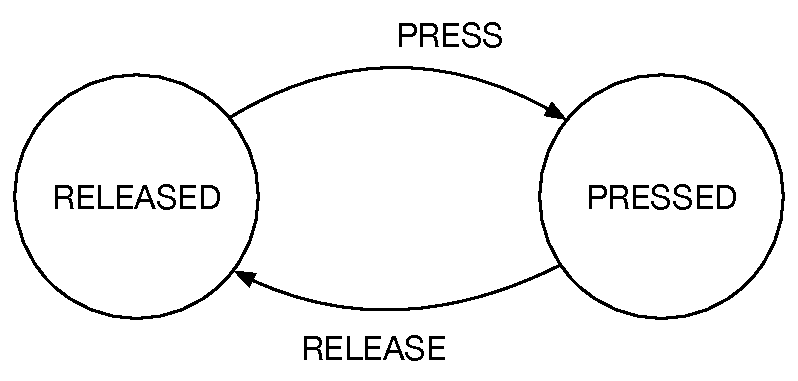
\includegraphics[height=6em]{button.pdf}
}
\end{figure}

To implement debouncing, I use a small array to keep track of the 3 most recent
values of \texttt{INT0}. Every 20 milliseconds, my debouncer pushes the most
recent value for \texttt{INT0} into this array and checks the values of each
element. If they are all equal to 1, it sends the \texttt{BUTTON\_PRESS} event
to my button FSM, and likewise for 0 and \texttt{BUTTON\_RELEASE}.\\

Below is a state diagram illustrating the FSM I use for detecting the morse code
pattern. It allows any sequence of dots and dashes to be pressed before the
desired pattern, and also loops back for prefixes as appropriate. Note that once
my FSM reaches its final accepting state, it will not continue to recognize
patterns; this is an intentional design choice, as the specification did not
state what the behaviour should be. The only behaviour in its state transition
function is to display ``CORRECT" when transitioning to the final state.

\begin{figure}[H]
\centering
\fbox{
    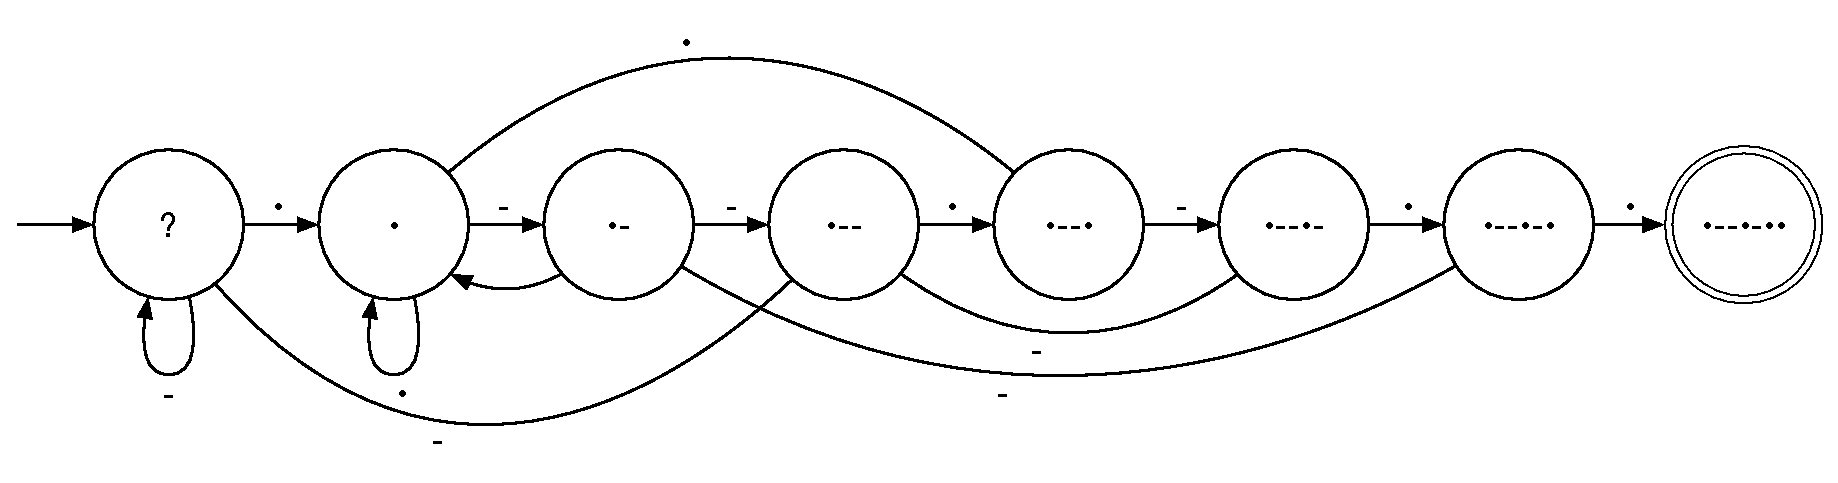
\includegraphics[width=\textwidth]{pattern.pdf}
}
\end{figure}

\end{document}
